\chapter{Algorithmen und Strukturen}
\label{cha:algorithmen}
% 7 Seiten

%supervised methoden: backpropagation
%unsupervised methoden: restricted boltzmann maschines, autoencoders, sparse coding model

\section{Backpropagation}

\begin{figure}
	\centering
	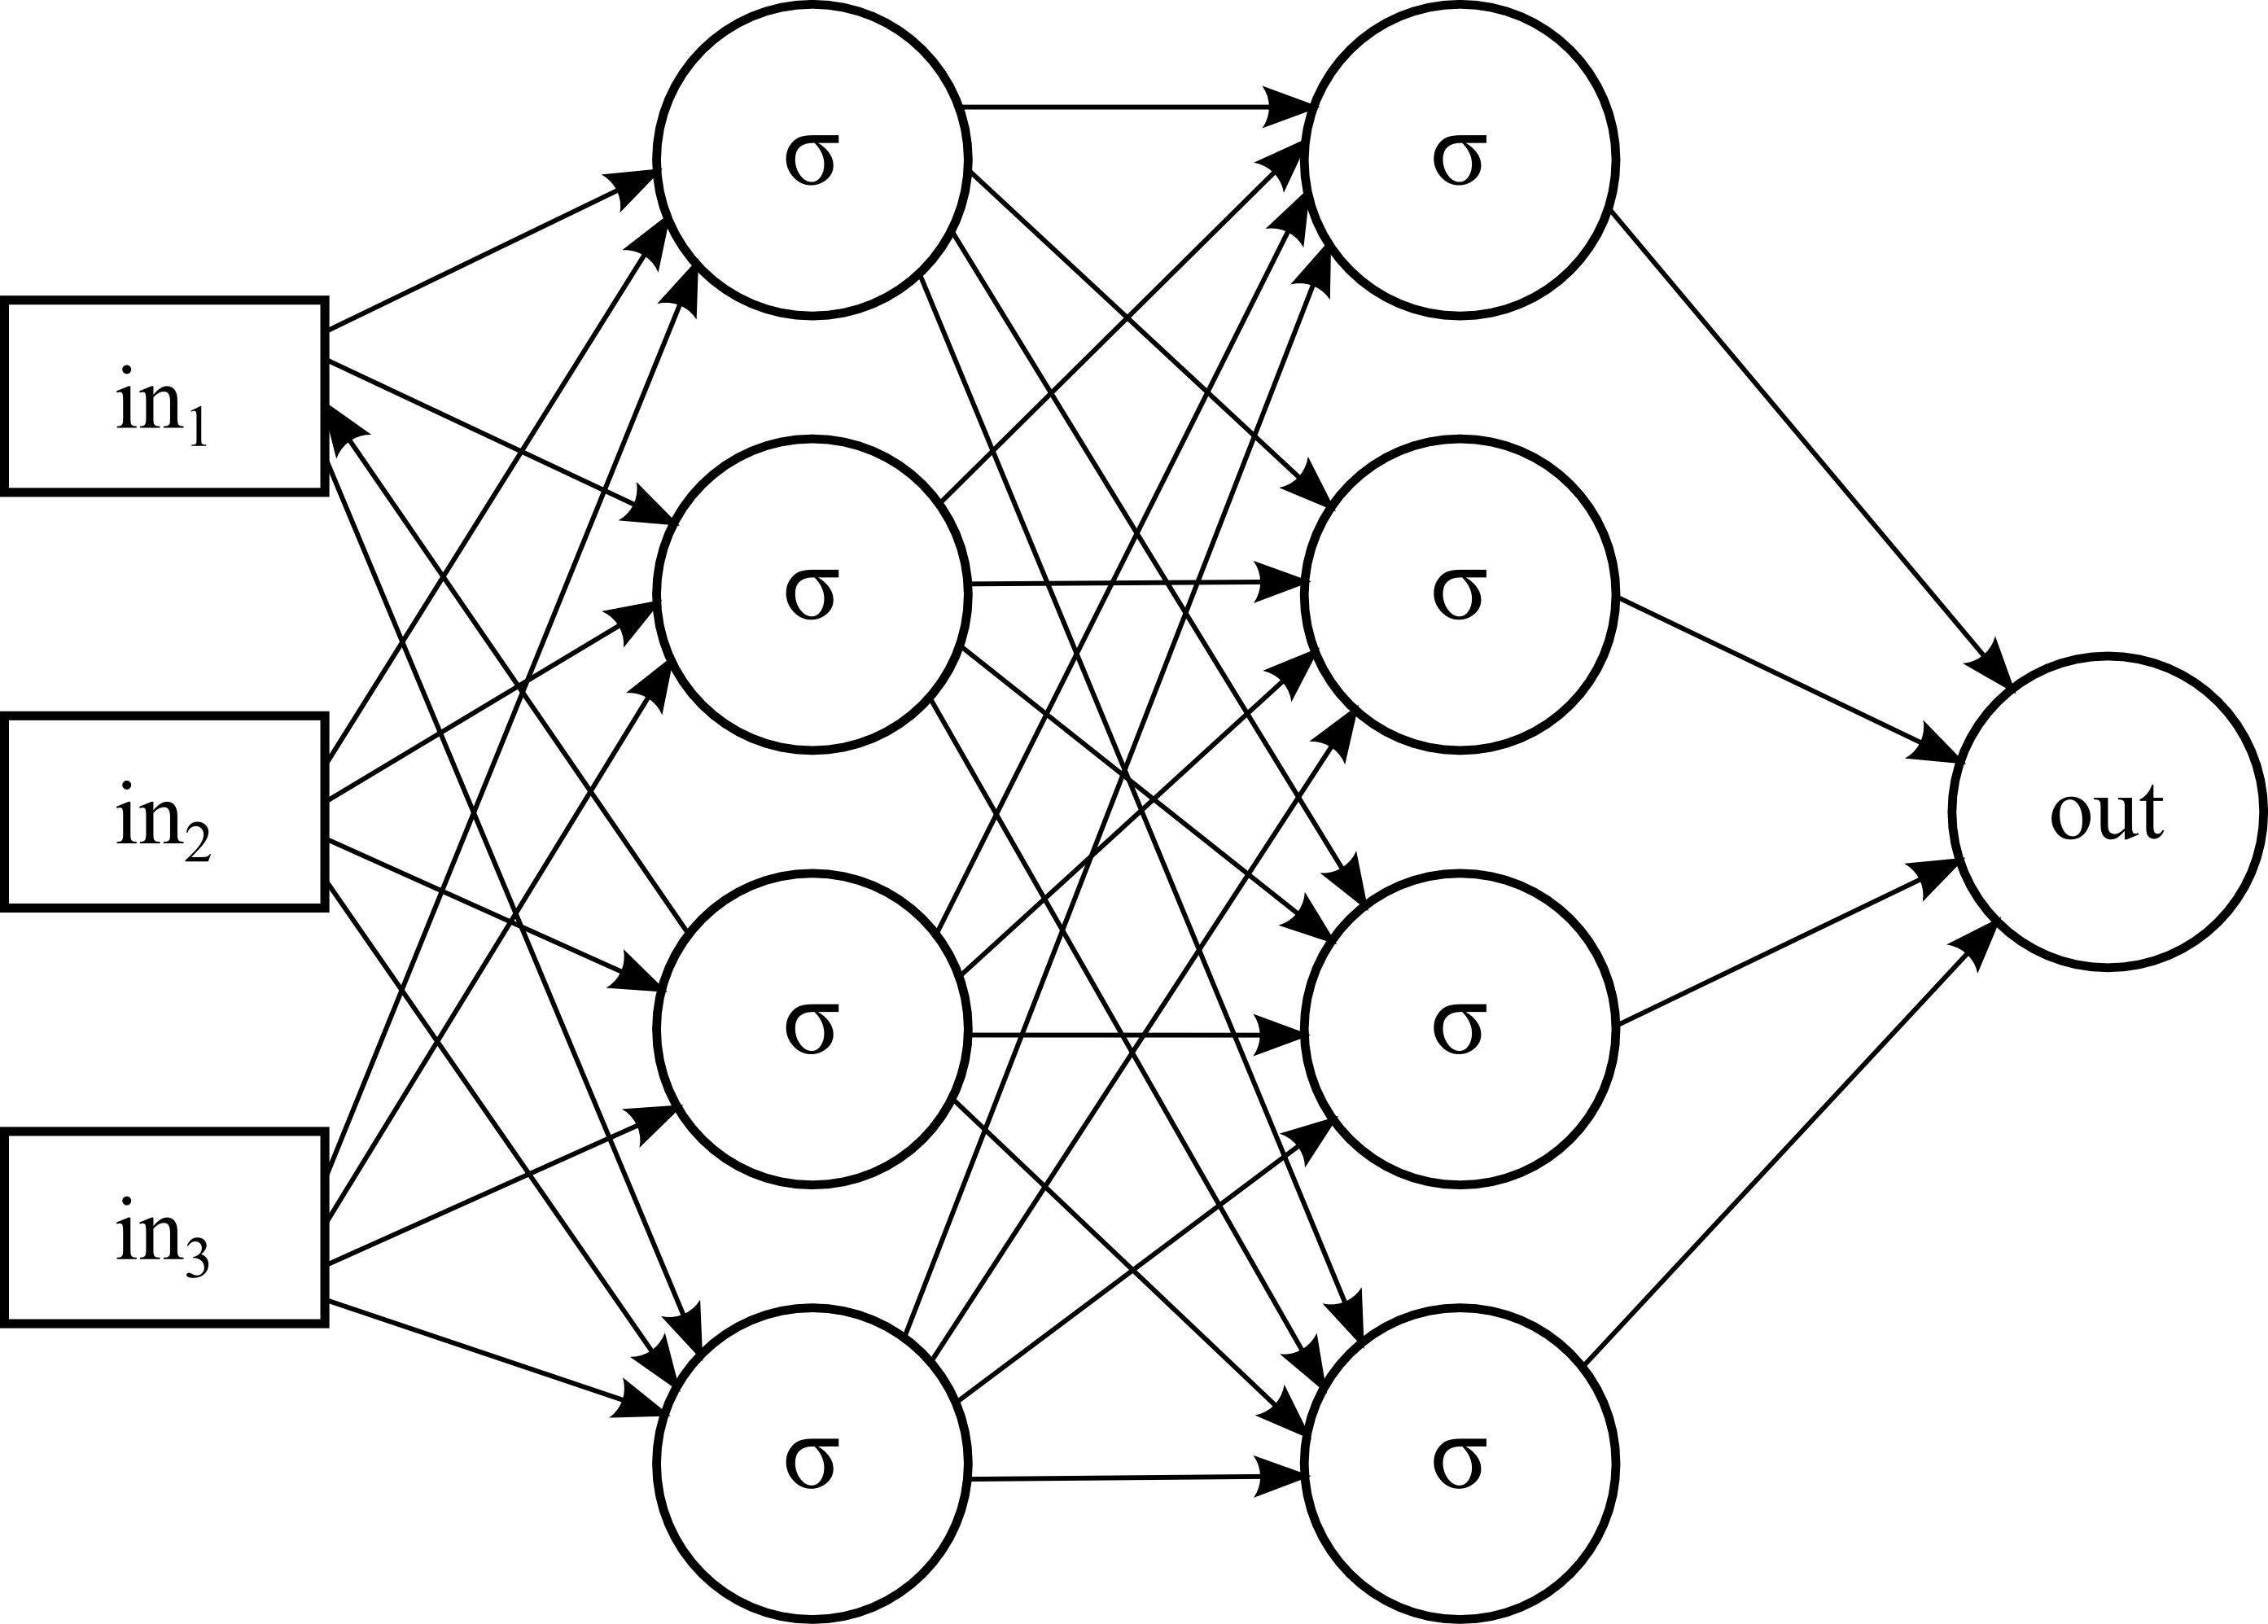
\includegraphics[scale=1]{images/net-for-bp.png}
	\caption{Ein Feedforward-Perzeptron}
	\label{fig:net-for-bp}
\end{figure}

Backpropagation ist ein überwachter Algorithmus zum Trainieren von vereinfachten neuronalen Netzen. Ein solches vereinfachtes Netz ist in Abbildung \ref{fig:net-for-bp} zu sehen und wird Feedforward-Perzeptrons genannt. Überwacht bedeutet, dass das Netzwerk beim Lernen anhand von deklarierten Eingabedaten, Ausgabedaten errechnet. Der Fehler der Berechnung des Ausgangs wird beim Backpropagation-Algorithmus über lineare Algebra zur Adaptierung der Gewichte genutzt.

Der Trainingsprozess beginnt mit zufälligen Gewichten und arbeitet in den folgenden Schritten:

\begin{enumerate}
\item Ausgang des Netzes für bestimmte Eingabedaten berechnen
\item Ausgang mit dem Sollwert vergleichen und daraus den Fehler errechnen
	$$error = \frac{1}{K}\sum_{k \in K}(out_k-target_k)^2$$
	\begin{center}\begin{tabular}{rclcrcl}
		$error$ & \dots & Fehler, der später Einfluss in die Gewichte nimmt\\
		$out$ & \dots & Wert den der Ausgang erreicht hat\\
		$target$ & \dots & Wert den der Ausgang erreichen sollte\\ 
		$K$ & \dots & Anzahl der Neuronen in der Ausgangsschicht\\
	\end{tabular}\end{center}
\item Gewichte abhängig von der Größe des Fehlers anpassen
\end{enumerate}

Diese Schritte werden wiederholt, bis die Gewichte so angepasst wurden, dass die Ausgangsdaten möglichst gut den Vorgaben entsprechen oder eine maximale Anzahl von Iterationen erreicht ist. Die Anpassung der Gewichte errechnet sich im wesentlichen anhand der Gradienten des Fehlers und der Gewichte. Zudem wird die Tiefe der Schicht des Gewichtes berücksichtigt.

\begin{figure}
	\centering
	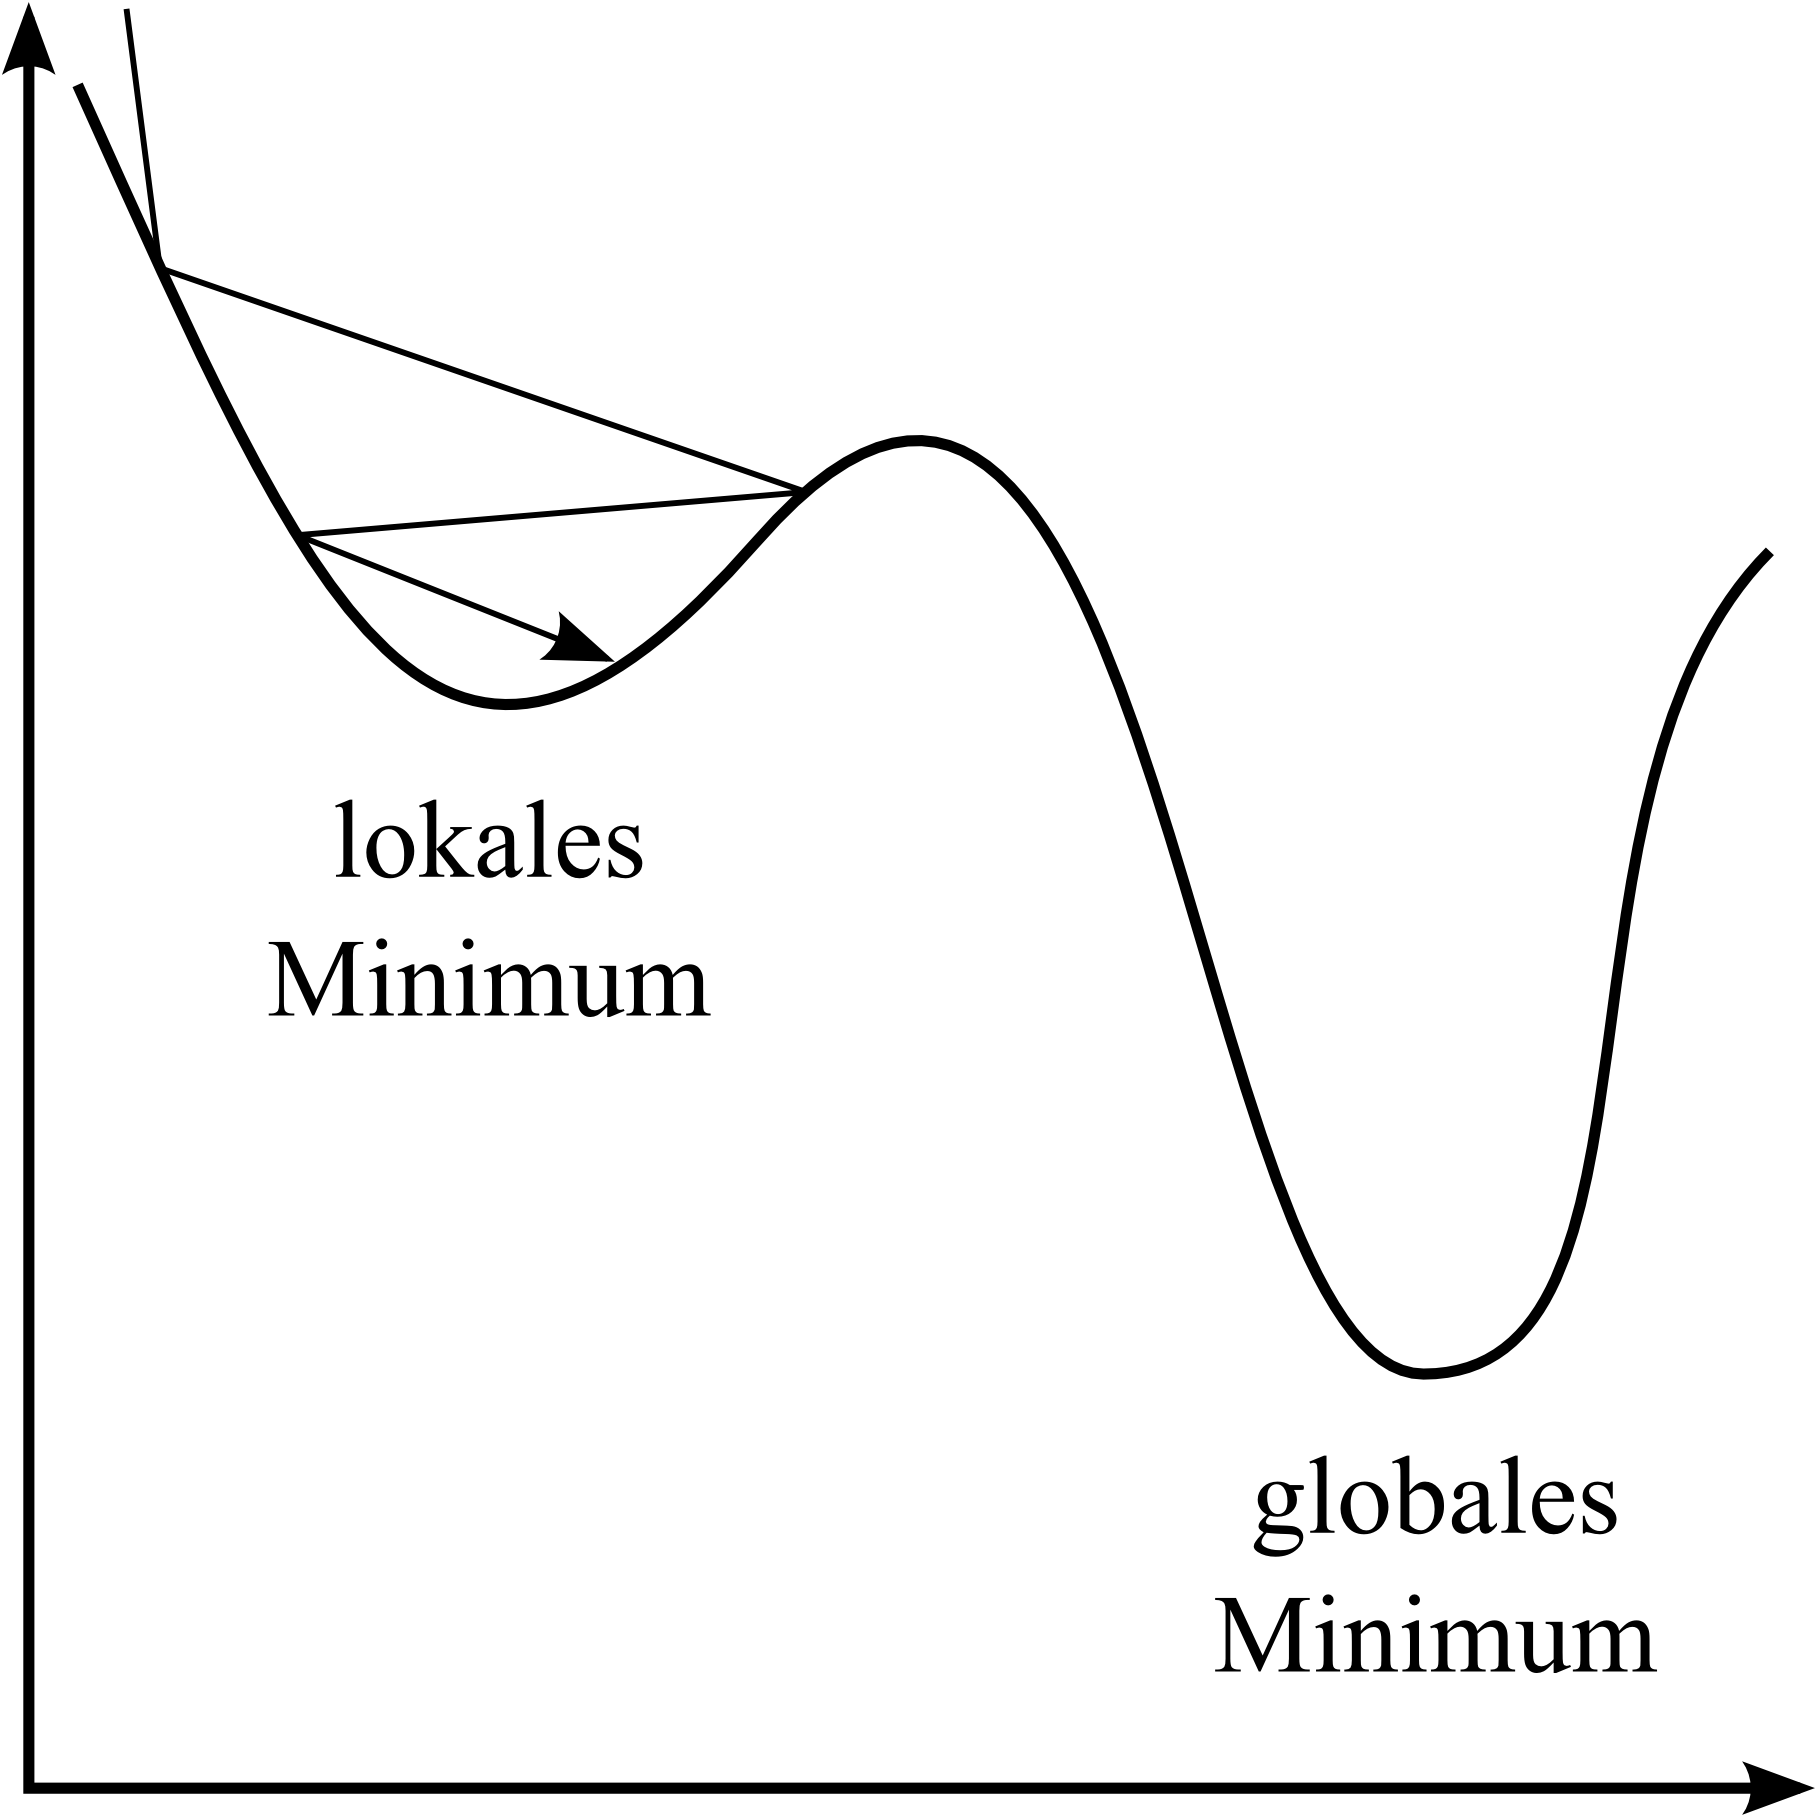
\includegraphics[scale=1]{images/lokales-minimum.png}
	\caption{Lokales Minimum}
	\label{fig:local-min}
\end{figure}

Wie der Name des Algorithmus bereits verrät, wird der Fehler dabei im wesentlichen über eine mathematische Funktion in die Gewichte zurückgeführt. Diese Rückführung bringt das Problem von lokalen Minima mit sich. Wird die Änderung des Fehlers geringer, so wird auch die Anpassung geringer. Befindet man sich auf dem Weg zu einem lokales Minimum, so kann man durch den abnehmenden Fehler, wie in Abbildung \ref{fig:local-min} zu sehen, leicht darin hängen bleiben. Dieses lokale Minimum kann sehr weit von dem globalen Minimum entfernt sein. Die Wahrscheinlichkeit in dem lokalen Minimum hängen zu bleiben steigt mit seiner Größe. Abhilfe kann hier der Neustart mit zufälligen Initialgewichten schaffen.

Der Algorithmus trainiert das Netz mit vordefinierte Ein- und Ausgabedaten mit dem Ziel für ähnliche Daten ähnliche Ergebnisse zu liefern. Trainiert man das Netz zu intensiv mit diesen Daten, so lernt es sie sehr genau. Dieser Effekt wird Überanpassung genannt und hat zur Folge, dass das Netz im späteren Betrieb schlechtere Ergebnisse liefert als hätte man es weniger lange trainiert. Abhilfe kann hier ein verfrühtes Ende des Trainings, mehr Trainingsdaten oder die Initialisierung der Gewichte durch unüberwachtes Lernen schaffen.

\section{Restricted Boltzmann Maschines}

\begin{figure}
	\centering
	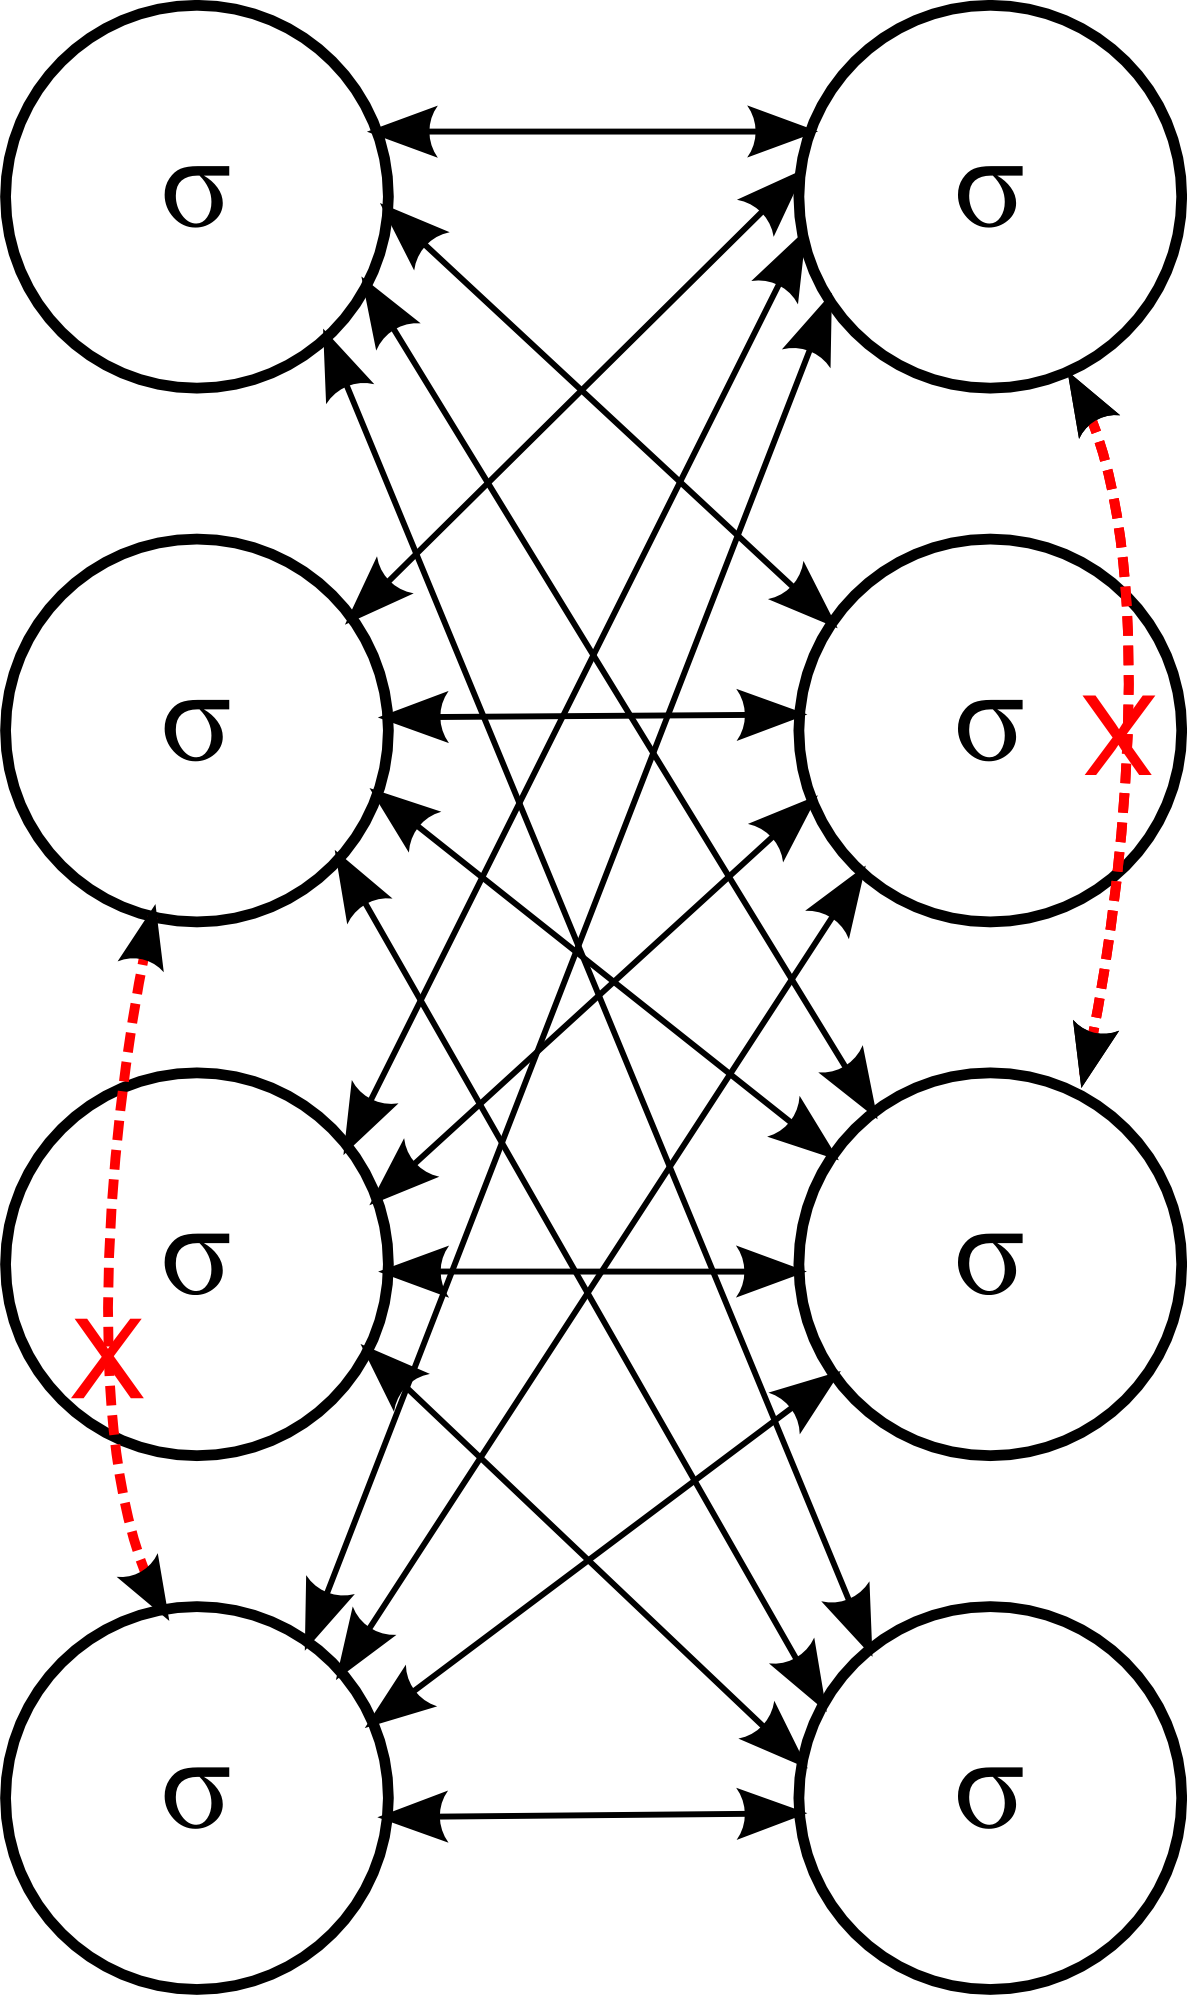
\includegraphics[scale=1]{images/rbm.png}
	\caption{Eine Restricted Boltzmann Maschine}
	\label{fig:rbm}
\end{figure}

Neuronale Netze ohne Einschänkungen der Verbindungen sind schwierig und aufwendig zu trainieren. Restricted Boltzmann Maschinen, im weiteren als RBMs bezeichnet, sind eingeschränkte neuronale Netzwerke. Wie in Abbildung \ref{fig:rbm} dargestellt, existieren hierbei nur Verbindungen zwischen aneinander liegenden Schichten. Das Modell erlaubt keine Verbindungen von Neuronen zu sich selbst und alle Verbindungen müssen gleichermaßen in beide Richtungen verlaufen. So lässt sich unter Festlegung der Werte einer Schicht direkt auf die nächste versteckte Schicht weiter rechnen. RBMs arbeiten in der Regel mit Bool'schen Werten, lassen sich durch Erweiterung aber auch mit anderen Zahlenräumen verwenden.

RBMs wurden bereits 1986 von Paul Smolensky \citep{rbm} unter dem Namen Harmonium erfunden, fanden jedoch erst 1998, rund 10 Jahre später, durch die Entwicklung von effizienten Lernalgorithmen durch Geoffrey Hinton Anwendung.

Zum Trainieren von RBMs existieren verschiedene Algorithmen, die meist auf dem Prinzip beruhen, die Gewichte so anzupassen, dass das hin und her Rechnen zwischen zwei Schichten wieder die Ausgangsdaten ergibt. Im folgenden wird der Algorithmus von Geoffrey Hinton \citep{BackpropagationFast}, der zugleich als der erste effizienten Lernalgorithmus für RBMs gesehen wird, erklärt.

\subsection{Grundgedanke}

\begin{figure}%
\centering
\subfloat[Versteckte Schicht berechen]{\begin{minipage}{0.33\textwidth}\centering%
	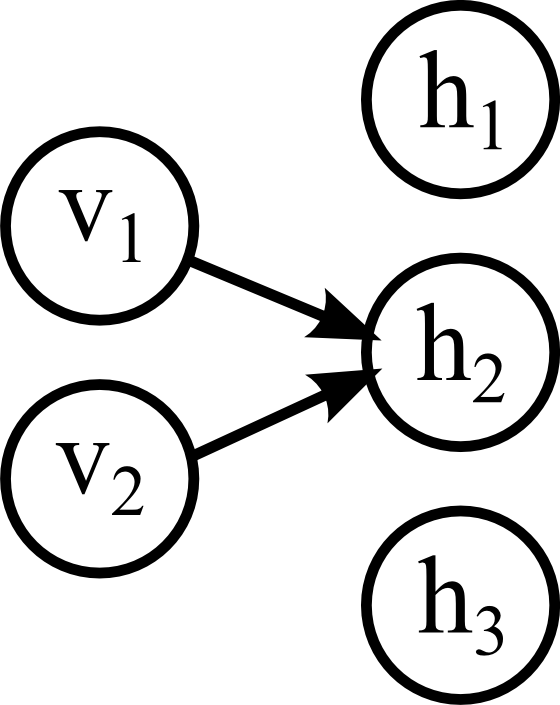
\includegraphics[scale=1]{images/rbm-step1.png}\end{minipage}}
\subfloat[Von der versteckten Schicht zurück rechnen]{\begin{minipage}{0.33\textwidth}\centering%
	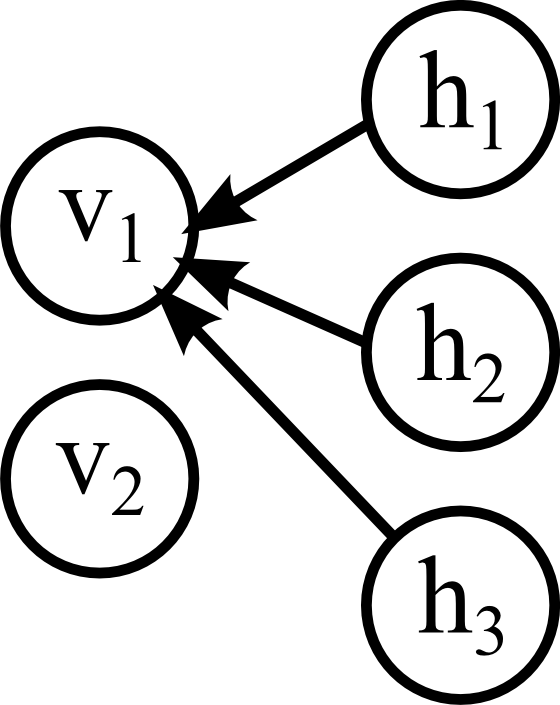
\includegraphics[scale=1]{images/rbm-step2.png}\end{minipage}}
\subfloat[Erneut die versteckte Schicht berechnen]{\begin{minipage}{0.33\textwidth}\centering%
	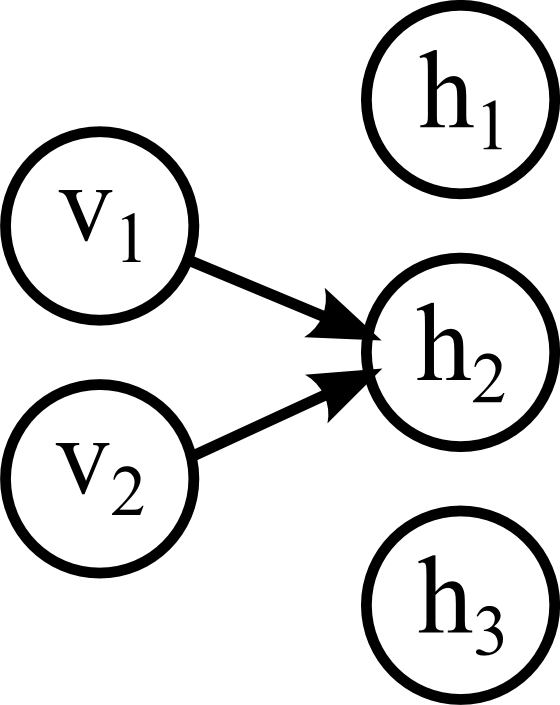
\includegraphics[scale=1]{images/rbm-step3.png}\end{minipage}}
\caption{Berechnungsschritte zum Lernen von RBMs.}
\label{fig:rbm-steps}
\end{figure}

Sind die Werte einer Schicht fixiert, so kann einfach auf die nächste versteckte Schicht weiter gerechnet werden. Zu Beginn werden ein Trainingsdatenset an die Eingänge angelegt und die folgenden Operationen, wie auch in Abbildung \ref{fig:rbm-steps} zu sehen, wiederholt ausgeführt:

\begin{enumerate}
\item Wahrscheinlichkeit $p$ für die versteckten Neuronen $h_j$ anhand der sichtbaren Neuronen $v_i$ und der Gewichte $w_{ij}$ berechnen $$p(h_j=1) = \frac{1}{1+e^{-(b_j+\sum_{i}(v_i*w_{ij}))}}$$
\item Gradientenmatrix $<v_ih_j>$ über das dyadische Produkt errechnen $$<v_ih_j> = v*y^T$$
\item Ausgehend von den errechneten versteckten Neuronen, zurück auf die sichtbare Schicht rechnen
\end{enumerate}

Wiederholt man die in der Liste angeführten Schritte sehr oft, so pendeln sich für die Neuronen Werte ein. Diese Werte hängen im wesentlichen vom Modell und den festgelegten Wahrscheinlichkeiten ab, haben jedoch sehr wenig mit den Eingangsdaten zu tun. Anhand der Gradientenmatrix des letzten Durchlaufes lässt sich jedoch eine Differenz zu dem gesuchten Modell herausfinden und so können die Gewichte wie folgt angepasst werden:
$$\Delta\omega_{ij} = \varepsilon (<v_ih_j>^0 -  <v_ih_j>^\infty)$$

Diese Art der Ergebnisse lieferte sehr gute Modelle. Durch die vielen Iterationen benötigt der Algorithmus sehr viel Rechenzeit und ist daher nicht praxistauglich. Zudem ist es schwierig festzustellen, wie viele Iterationen notwendig sind bis sich die Werte eingependelt haben.

\subsection{Abkürzung}

Der oben genannte Algorithmus lässt sich in seiner Komplexität erheblich reduzieren, in dem die versteckte Schicht lediglich zwei mal berechnet wird. Geoffrey Hinton hat mit der Vereinfachung gezeigt, dass es bereits mit dem Vergleich der ersten und zweiten Gradientenmatrix möglich ist, gute Ergebnisse zu erzielen \citep{ContrustiveDivergence}. Diese Methode wird \emph{Contrastive Divergence} genannt.

Die Regel zur Anpassung der Gewichte lautet dabei:
$$\Delta\omega_{ij} = \varepsilon (<v_ih_j>^0 -  <v_ih_j>^1)$$

\subsection{Begründung}

Der Grundgedanke von \emph{Contrastive Divergence} ist es, dass das Modell mit Zufallsgewichten weg von den Eingabedaten, hin zu Daten die ihm besser gefallen, wandert. Wenn man erkennt wo hin das Modell will, kann man die Gewichte so adaptieren, dass das Modell zu den Eingabedaten will.

\subsection{Eignung}

Der Algorithmus benötigt extrahiert aus den nicht deklarierten Eingabedaten Merkmale die die Daten klassifizieren. Er eignet sich daher um Gemeinsamkeiten und von Eingabedaten, wie zum Beispiel Bildern, zu finden.

\section{Deep Autoencoders}

\begin{figure}
	\centering
	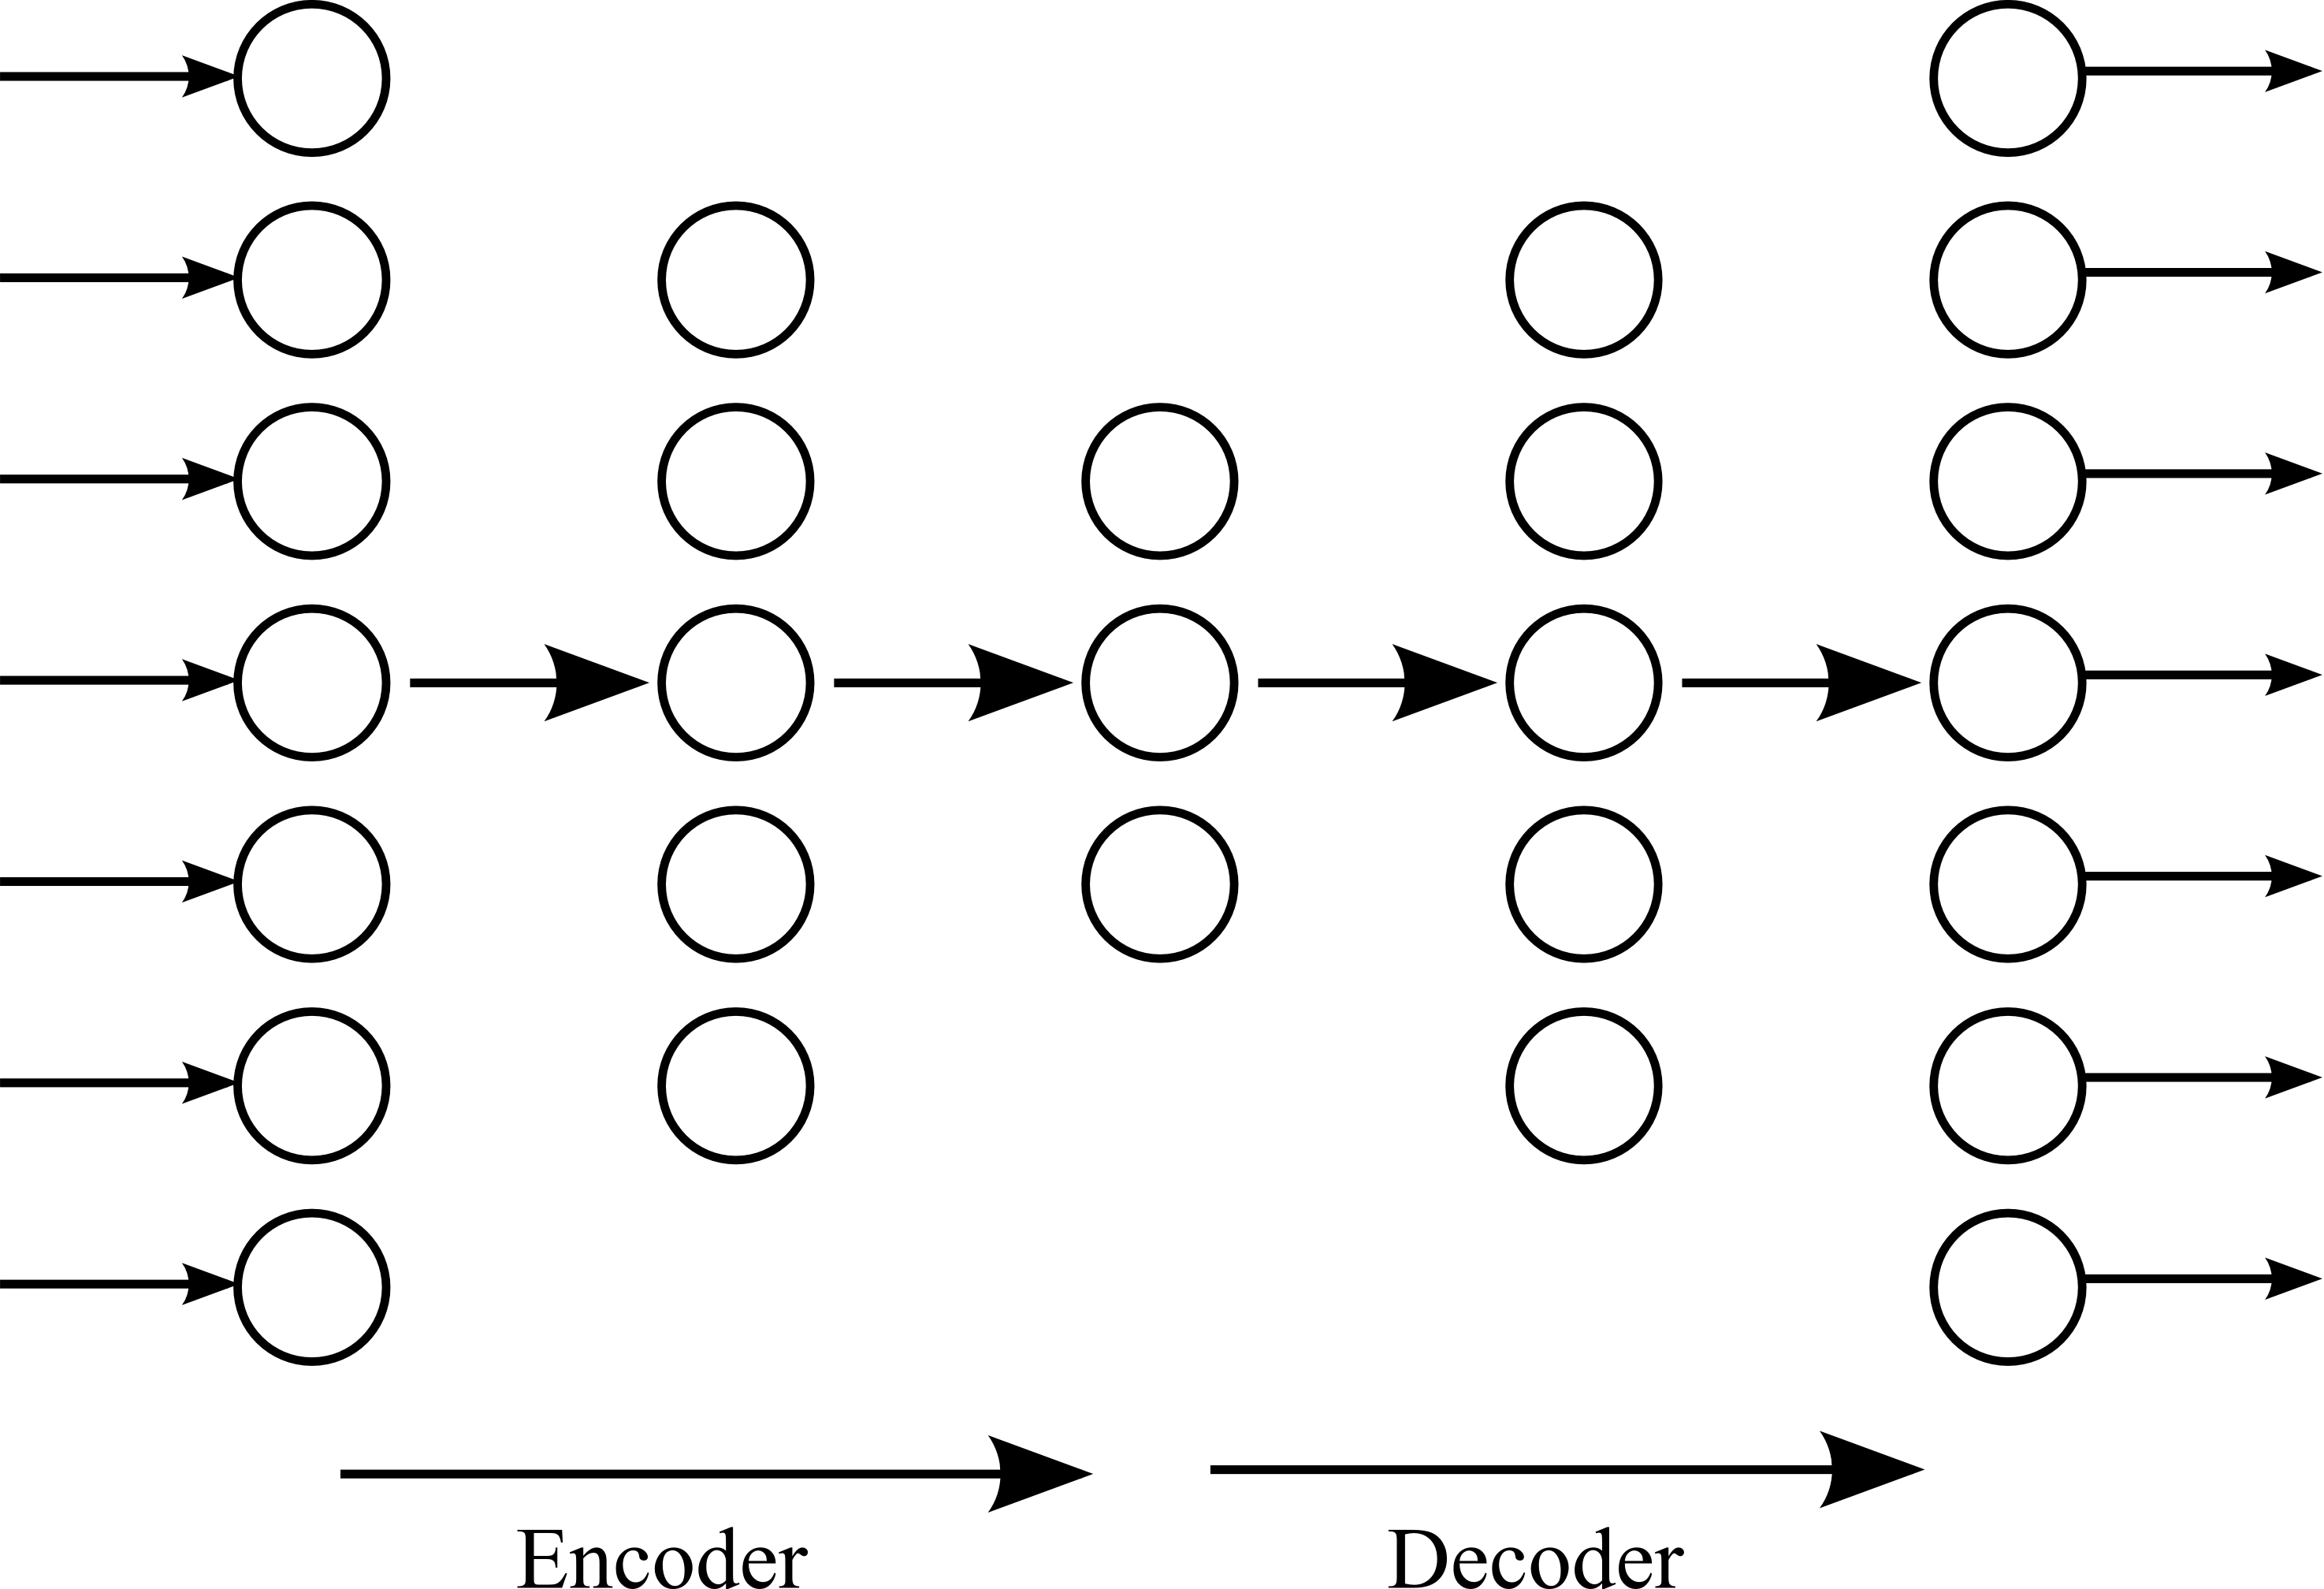
\includegraphics[scale=1]{images/autoencoder.png}
	\caption{Deep Autoencoder}
	\label{fig:autoencoder}
\end{figure}

Deep Autoencoder sind neuronale Netze aus mehreren Schichten, die sich in zwei wesentliche Teile trennen lassen. Im ersten Teil, dem Encoder, sinkt die Anzahl der Neuronen mit jeder Schicht. Im zweiten Teil, dem Decoder, steigt sie, bis am Ende wieder die Anzahl der Eingangsparameter erreicht ist. Abbildung \ref{fig:autoencoder} zeigt ein solches Netz. Im inneren hat das Netz weniger Neuronen und somit geringere Speicherkapazität als Eingangsparameter. Es wird versucht das Netz so zu trainieren, dass es am Ausgang die gleichen Daten berechnet wie am Eingang angelegt entstehen. Gelingt das Training, so muss das Netz Merkmale etwas aus den Daten gelernt haben.

Richtig trainiert, komprimiert das Netz die Daten. So wäre es zum Beispiel möglich Bilder durch das Netz zu schicken, die kleinste Schicht zu speichern und jederzeit über den Decoder wiederherzustellen. Für Bilder, Ton und Videos gibt es einige Kompressionsalgorithmen die sehr fein auf die Charakteristik menschlicher Organe abgestimmt sind und Dinge die wir nicht hören oder Sehen können vernachlässigen. Diese Algorithmen liefern für diesen Anwendungsfall daher meist bessere Ergebnisse. Dennoch demonstriert das Beispiel, dass damit unter Umständen erheblich Speicher und Verarbeitungsleistung eingespart werden kann werden kann. Oft entsprechen die Daten der Dekodierung sogar mehr dem gewünschten Ergebnis als zuvor. Ein Netzt das darauf trainiert ist Buchstaben zu lesen, könnte man zum Beispiel im inneren so klein machen, dass es lediglich die einzelnen Buchstaben ohne Manipulationen speichern kann. Beim wiederherstellen würde es dann den Buchstaben erzeugen der seinem Muster am besten entspricht.

Deep Autoencoder liefern sehr vergleichbare Ergebnisse und werden daher gerne als Benchmark für Deep Learning-Algorithmen verwendet \citep{AutoencoderBenchmark}. Deep Autoencoders tendieren zu Unteranpassung (eng. underfitting), was auf die geringe Anzahl der Neuronen und damit der geringen Speichermöglichkeit zurückzuführen ist. Eine einfache und effektive Variante ein solches Netz zu trainieren ist es, jeweils zwei Layer separat als restricted Boltzmann Maschine anzusehen.

Lernt man solche Algorithmen mit mit Bildern und visualisiert die entstandenen Gewichte, so erkennt man, dass solche Algorithmen in erster Instanz meist Kanten und Farbintensitäten finden. In der zweiten Schicht findet man einfache Kombinationen dieser Elemente und ab der dritten Schicht werden meist schon sehr brauchbare Neuronen zur vollständigen Objekterkennung ausgebildet.

\section{Faltungscodierte neurale Netze}
% als grundlage

Faltungskodierte neuronale Netze \footnote{eng. Convolutional Neural Networks} sind neuronale Netze, die zur Reduktion der Gewichte in einzelne Teile zerteilt sind. Bei den bisher angeführten Netzen wurden jeweils alle Neuronen einer Schicht mit jedem Neuron der nächsten Schicht verbunden. Bei faltungskodierten Netzen geht man davon aus, dass weit voneinander entfernte Neuronen kaum etwas miteinander zu tun haben, während zwischen nahe aneinander liegende Neuronen Zusammenhänge bestehen. Es werden daher Gruppen von aneinanderliegenden Neuronen gebildet. Dies Gruppen sind untereinander in die nächste Schicht verknüpft. Wie am Beispiel eines Bildes gut verständlich, wird es vorkommen, dass ein Merkmal nicht genau in eine dieser Gruppen passt. Es werden daher viele überlappende Gruppen gebildet.

\begin{figure}
	\centering
	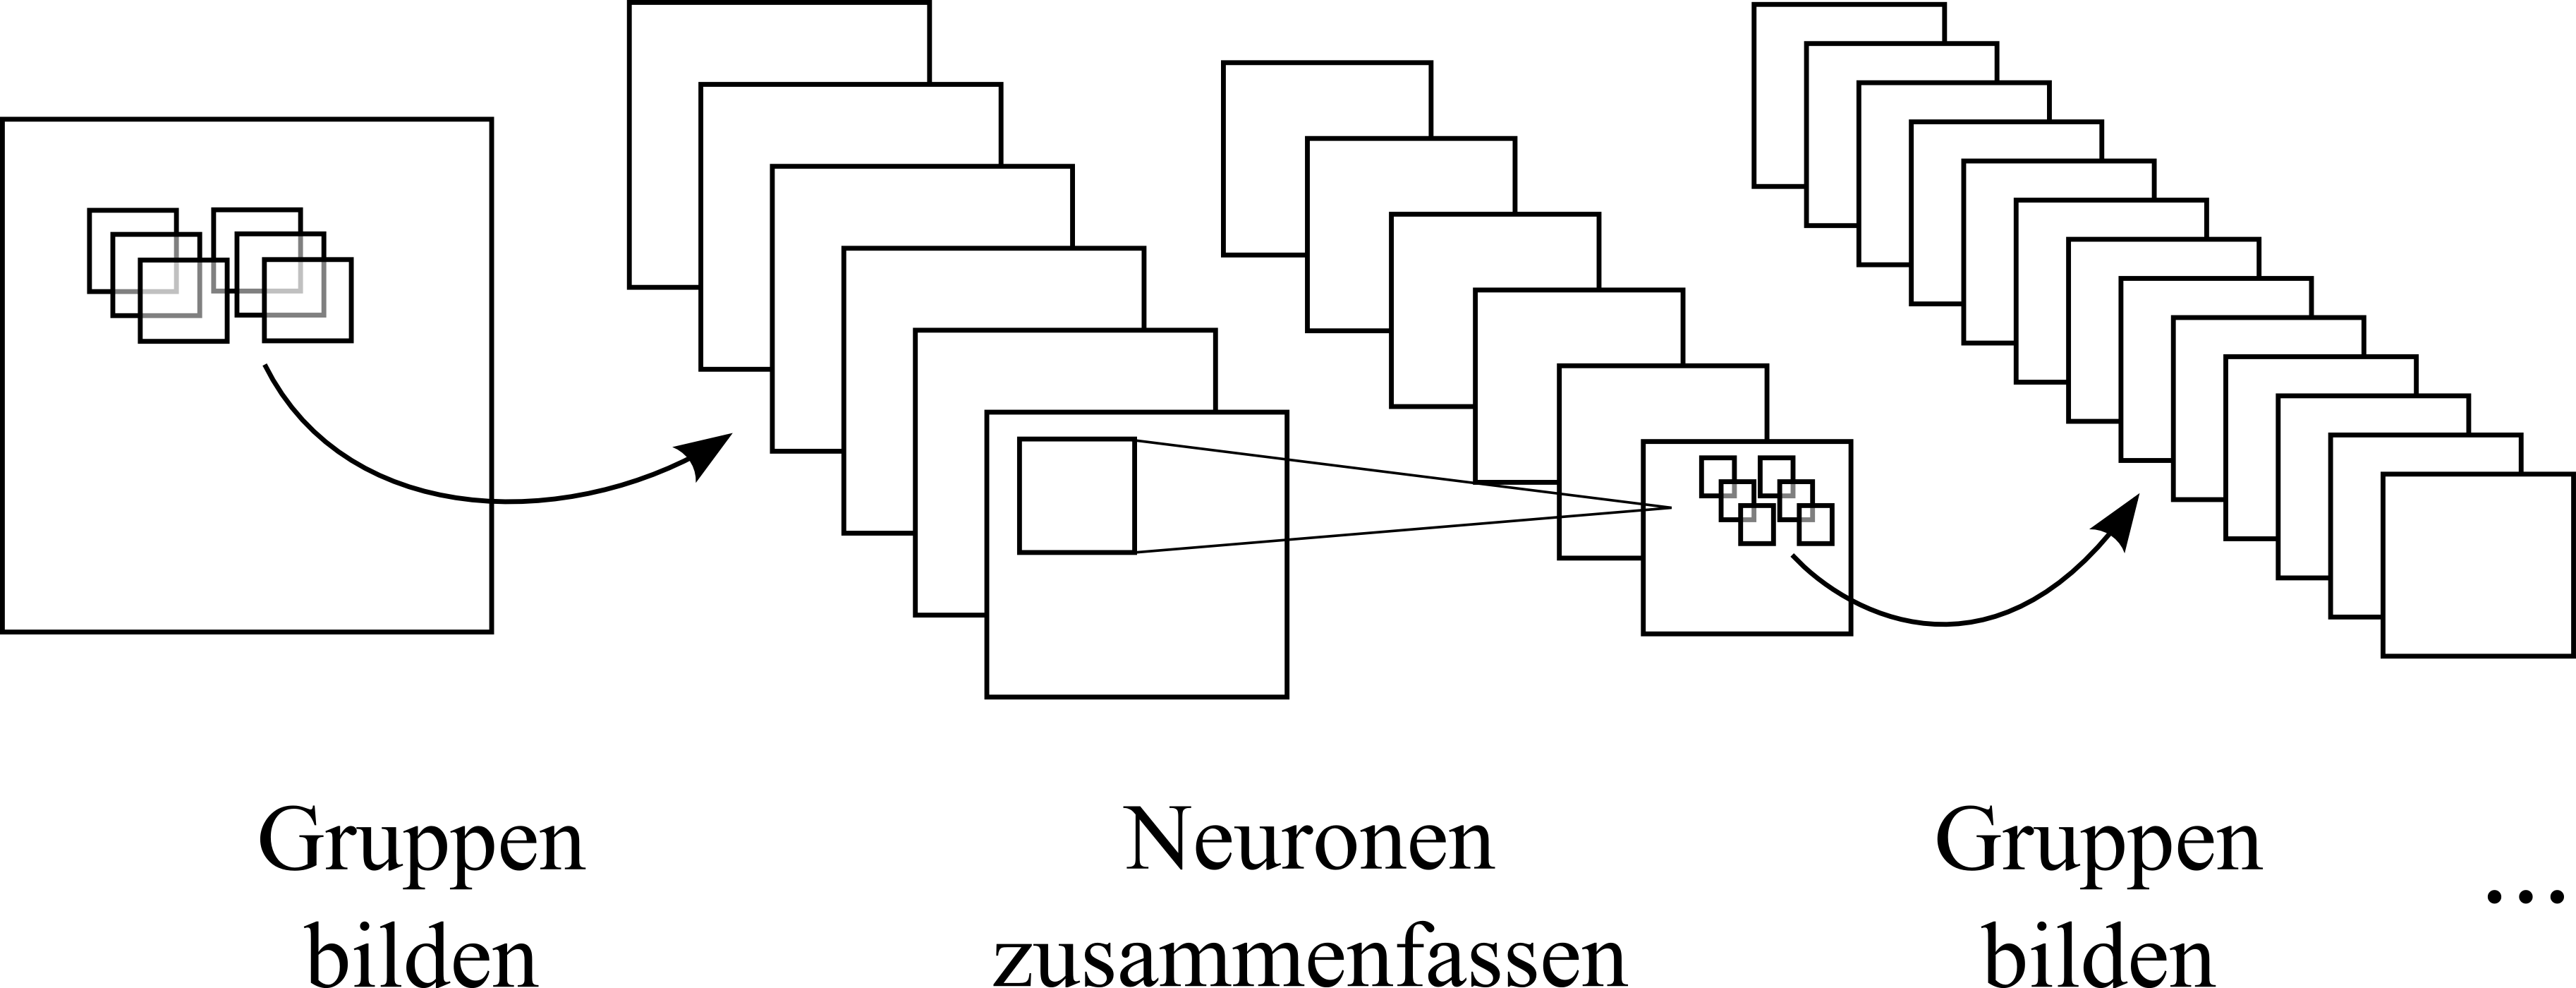
\includegraphics[scale=1]{images/convolution.png}
	\caption{Faltungscodiertes neuronales Netz}
	\label{fig:convolution}
\end{figure}

Nach der Gruppenbildung gibt es eine Funktion, die die Ergebnisse aneinander liegender Werte für die nächste Schicht zusammenfasst. Dies geschieht meist über eine einfache mathematischen oder statistische Funktion und hängt von der Implementierung ab. Diese Funktion könnte zum Beispiel die Kanten in mehrere Richtungen zusammenfasse um die Rotation eines Bildes ignorieren.

Ein faltungskodiertes neuronales Netz wiederholt genau diesen zwei Komponenten, die überlappende Gruppierung von Neuronen so wie das zusammenfassen von Neuronen auf jeder Schicht. Abbildung \ref{fig:convolution} zeigt ein solches Netz.

Dieser Typ von Netzwerk ist bereits 1980 \citep{convolutional} bekannt, wurde in den folgenden Jahrzehnten optimiert und erlebte einen Aufschwung durch die parallelisierte Berechnung auf einer GPU \citep{dandan}. Nach weiteren Optimierungen in den vergangen Jahren wurde ein solches Netzwerk unter anderem für ein Projekt von Google \citep{googleimage} eingesetzt, das nicht zuletzt das so genannte face-Neuron ausprägte.

\section{Sparse coding}

Sparse coding ist ein Algorithmus zum trainieren eines neuronalen Netzes mit dem Ansatz möglichst aussagekräftige Merkmale zu finden. Anders als beim Deep Autoencoder wird hier nicht nur berücksichtigt wie gut das Ergebnis wiederhergestellt werden konnte, sondern auch wie eindeutig das Ergebnis war. Ziel ist es an möglichst vielen Stellen im Ausgangsvektor den Wert Null zu berechnen und dennoch sehr gute Ergebnisse zu finden. Die Zielfunktion setzt sich aus zwei Faktoren zusammen und wird wie folgt berechnet:

$$min\frac{1}{T}\sum_{t=1}^{T}\frac{1}{2}|x^{(t)}-D*h^{(t)}|+\lambda|h^{(t)}_1|$$
\begin{center}\begin{tabular}{rclcrcl}
	$x^{(t)}$ & \dots & Eingangswert\\
	$h^{(t)}$ & \dots & Ausgangswert\\
	$D$ & \dots & Anzahl der Ausgänge\\
	$\lambda$ & \dots & Faktor zur Gewichtung\\ 
\end{tabular}\end{center}

Die zwei zu minimierenden Bedingungen der Zielfunktion, Abweichung vom Ziel und die Zahl Nuller im Ergebnisvektor widersprechen sich teilweise und können über $\lambda$ balanciert werden. Die Berechnung der Gewichte für die versteckten Schichten ist beim Sparse Coding wesentlich aufwendiger als bei Deep Autoencodern, da es sich hier um ein Optimierungsproblem und nicht nur um eine lineare Funktion handelt.